\documentclass[11pt]{article}
\usepackage[T1]{fontenc}
\usepackage{lmodern}
\usepackage[margin=1in]{geometry}
\usepackage{amsmath,amssymb,amsthm,mathtools}
\usepackage{booktabs,graphicx,array,xcolor}
\usepackage[font=small,labelfont=bf]{caption}
\usepackage{placeins}
\renewcommand{\topfraction}{0.94}\renewcommand{\bottomfraction}{0.88}\renewcommand{\textfraction}{0.06}
\renewcommand{\floatpagefraction}{0.80}
\usepackage[numbers,sort&compress]{natbib}
\usepackage{microtype}
\definecolor{cosblue}{HTML}{1F4E8C}
\usepackage{xurl}
\usepackage[colorlinks=true,linkcolor=cosblue,citecolor=cosblue,urlcolor=cosblue]{hyperref}

\newcommand{\E}{\mathbb{E}}
\newcommand{\R}{\mathbb{R}}
\newcommand{\RP}{R_\Pi}
\newcommand{\dd}{\,\mathrm{d}}
\newcommand{\Var}{\operatorname{Var}}
\newcommand{\RoughCert}{\textsf{RoughCert}}
\newcommand{\RoughCertTilt}{\textsf{RoughCert-Tilt}}
\newcommand{\RoughCertCV}{\textsf{RoughCert-CV}}
\newcommand{\EfiveCells}{24}
\newcommand{\EfiveCertMin}{1.000}
\newcommand{\EfiveNaiveUnder}{11}
\newcommand{\EfiveNaiveZero}{4}
\newcommand{\EfiveRatioLo}{4}
\newcommand{\EfiveRatioHi}{53}
\newcommand{\EfiveFineNaiveLo}{0.940}
\newcommand{\EfiveFineNaiveHi}{0.965}
\newcommand{\EfiveFineN}{64}
\newcommand{\EfiveTruthDisc}{$2.2\times10^{-4}$}
\newcommand{\EfiveUnderEpsWide}{11}
\newcommand{\EfourCells}{24}
\newcommand{\EfourFeasible}{12}
\newcommand{\EfourGreedyLo}{1.0}
\newcommand{\EfourGreedyHi}{21.9}
\newcommand{\EfourSepLo}{2.0}
\newcommand{\EfourSepHi}{87.4}
\newcommand{\EfourUnifLo}{2.0}
\newcommand{\EfourUnifHi}{$1.2\times10^{5}$}
\newcommand{\EfourGreedyWithin}{2}
\newcommand{\EfourGreedyBeatsUnif}{8}
\newcommand{\EfourSepOver}{12}
\newcommand{\EfourOverspent}{10}
\newcommand{\EfourOvershootN}{9}
\newcommand{\EfourInvalid}{0}
\newcommand{\EfourBestLo}{11}
\newcommand{\EfourBestHi}{28}
\newcommand{\EfourGridLo}{8}
\newcommand{\EfourGridHi}{21}
\newcommand{\EsixCells}{12}
\newcommand{\EsixIssued}{0}
\newcommand{\EsixUnresolved}{12}
\newcommand{\EsixMCInside}{12}
\newcommand{\EsixMonLo}{8}
\newcommand{\EsixMonHi}{117}
\newcommand{\EsixHmin}{0.05}
\newcommand{\EsixHmax}{0.3}
\newcommand{\EsixMonRoughLo}{49}
\newcommand{\EsixMonRoughHi}{117}
\newcommand{\EsixMonSmoothLo}{8}
\newcommand{\EsixMonSmoothHi}{20}
\newcommand{\EsixBiasFloor}{12}
\newcommand{\EsixSampling}{0}
\newcommand{\EsixRouteD}{0}
\newcommand{\EsixIssuedList}{none}
\newcommand{\EnineGapMax}{$1.1\times10^{-9}$}
\newcommand{\EnineTanhNote}{The generic $\tanh(2y)$, supplied only as a function, was handled by the same code.}
\newcommand{\EsevenEarlyLo}{1.4}
\newcommand{\EsevenEarlyHi}{2.1}
\newcommand{\EsevenLateLo}{283}
\newcommand{\EsevenLateHi}{992}
\newcommand{\EsevenIntLo}{43}
\newcommand{\EsevenIntHi}{334}
\newcommand{\EsevencStatLo}{1.02}
\newcommand{\EsevencStatHi}{1.09}
\newcommand{\EsevencTameLo}{1.3}
\newcommand{\EsevencTameHi}{2.2}
\newcommand{\EsevencHorizonLo}{213}
\newcommand{\EsevencHorizonHi}{469}
\newcommand{\EsevencAuditMax}{$1.9\times10^{-7}$}
\newcommand{\EfourcCells}{28}
\newcommand{\EfourcRef}{24}
\newcommand{\EfourcMatched}{24}
\newcommand{\EfourcCrossMaxPct}{15}
\newcommand{\EfourcCrossMedPct}{1}
\newcommand{\EfourcInfeasNoCross}{14}
\newcommand{\EfourcInfeas}{14}
\newcommand{\EfourcTimeLo}{5}
\newcommand{\EfourcTimeHi}{95}
\newcommand{\EfourcTanhCells}{4}
\newcommand{\EfourcTanhSecHi}{6}
\newcommand{\EfivebCells}{12}
\newcommand{\EfivebCovMin}{1.00}
\newcommand{\EfivebRatioLo}{1.09}
\newcommand{\EfivebRatioHi}{1.93}
\newcommand{\EfivebRadLo}{1.00}
\newcommand{\EfivebRadHi}{1.31}
\newcommand{\EfivebMartLo}{1.09}
\newcommand{\EfivebMartHi}{1.47}
\newcommand{\EfivebNarrower}{12}
\newcommand{\EsixbCells}{12}
\newcommand{\EsixbIssued}{0}
\newcommand{\EsixbInside}{12}
\newcommand{\EsixbWidthLo}{0.34}
\newcommand{\EsixbWidthHi}{0.48}
\newcommand{\EsixbHalfLo}{44}
\newcommand{\EsixbHalfHi}{238}
\newcommand{\EsixbDailyLo}{0.41}
\newcommand{\EsixbDailyHi}{0.87}
\newcommand{\EpriceCells}{6}
\newcommand{\EpriceRatioLo}{1.1}
\newcommand{\EpriceRatioHi}{3.1}
\newcommand{\EpriceRelLo}{41}
\newcommand{\EpriceRelHi}{331}
\newcommand{\EpriceDailyOut}{0}
\newcommand{\EpriceFineIn}{6}
\newcommand{\ElevenStation}{12}
\newcommand{\ElevenCE}{8}
\newcommand{\ElevenCEnoisy}{29}
\newcommand{\ElevenCEnoisyFifty}{22}
\newcommand{\ElevenPlugin}{10}
\newcommand{\ElevenPluginNoisy}{38}
\newcommand{\ElevenPlugBias}{16}
\newcommand{\ElevenQlo}{0.316}
\newcommand{\ElevenQhi}{0.730}
\newcommand{\ElevenQmc}{0.500}
\newcommand{\EeightbQLo}{1.28}
\newcommand{\EeightbQHi}{1.49}
\newcommand{\EeightbESLo}{2.0}
\newcommand{\EeightbESHi}{2.1}
\newcommand{\EeightbTotLo}{2.2}
\newcommand{\EeightbTotHi}{3.4}
\newcommand{\EeightbIVes}{$[4.41,6.15]$}
\newcommand{\EtwelveOccQ}{91}
\newcommand{\EtwelveOccH}{43}
\newcommand{\EtwelveOccOne}{21}
\newcommand{\EtwelveOccTwo}{11}
\newcommand{\EtwelveSqQ}{61}
\newcommand{\EtwelveSqOne}{0.3}
\newcommand{\EtwelveExcTwo}{1.3}
\newcommand{\EtwelveOccSd}{0.010}
\newcommand{\EtwelveOccMean}{0.0478}
\newcommand{\EtwelveQlo}{0.0580}
\newcommand{\EtwelveQhi}{0.0735}
\newcommand{\EtwelveQc}{0.0650}
\newcommand{\EcantLo}{1.6}
\newcommand{\EcantHi}{2.1}
\newcommand{\EcantMartLo}{1.15}
\newcommand{\EcantMartHi}{1.36}
\newcommand{\EfivecCells}{12}
\newcommand{\EfivecCovMin}{1.00}
\newcommand{\EfivecCdLo}{1.16}
\newcommand{\EfivecCdHi}{1.58}
\newcommand{\EfivecAdLo}{1.26}
\newcommand{\EfivecAdHi}{2.37}
\newcommand{\EfivecRbLo}{1.05}
\newcommand{\EfivecRbHi}{1.26}
\newcommand{\EfivecNarrower}{12}
\newcommand{\EfivecExLo}{1.2}
\newcommand{\EfivecExHi}{6.6}
\newcommand{\EfivecFloorGap}{3}
\newcommand{\Efivecrbeps}{0.0120}
\newcommand{\Efivecdkweps}{0.0096}
\newcommand{\ESolveMartN}{256}
\newcommand{\ESolveMartK}{200{,}000}
\newcommand{\ESolveMartW}{0.293}
\newcommand{\ESolveMartSec}{243}
\newcommand{\ESolveMartIn}{yes}
\newcommand{\ESolveCvN}{64}
\newcommand{\ESolveCvK}{200{,}000}
\newcommand{\ESolveCvW}{0.243}
\newcommand{\ESolveCvSec}{48}
\newcommand{\ESolveCvIn}{yes}
\newcommand{\ESolveOsN}{64}
\newcommand{\ESolveOsK}{50{,}000}
\newcommand{\ESolveOsW}{0.219}
\newcommand{\ESolveOsSec}{48}
\newcommand{\ESolveOsIn}{yes}
\newcommand{\EfivecBinCov}{0.96}
\newcommand{\EfivecBinLo}{1.13}
\newcommand{\EfivecBinHi}{2.99}
\newcommand{\EfivecBinCLo}{1.34}
\newcommand{\EfivecBinCHi}{3.49}
\newcommand{\EfivecBinALo}{2.58}
\newcommand{\EfivecBinAHi}{4.25}
\newcommand{\EfivecBinCheck}{yes}
\newcommand{\EfivecSlopeCa}{0.38}
\newcommand{\EfivecSlopeDa}{0.54}
\newcommand{\EfivecPredCa}{1.08}
\newcommand{\EfivecPredDa}{1.08}
\newcommand{\EfivecNmaxa}{128}
\newcommand{\EfivecSlopeCb}{0.36}
\newcommand{\EfivecSlopeDb}{0.53}
\newcommand{\EfivecPredCb}{1.02}
\newcommand{\EfivecPredDb}{1.04}
\newcommand{\EfivecNmaxb}{128}
\newcommand{\EthirteenCells}{3}
\newcommand{\EthirteenKLvar}{0.12}
\newcommand{\EthirteenCovMin}{1.00}
\newcommand{\EthirteenWdLo}{0.71}
\newcommand{\EthirteenWdHi}{3.45}
\newcommand{\EthirteenCdLo}{1.56}
\newcommand{\EthirteenCdHi}{2.25}
\newcommand{\EthirteenAdLo}{2.46}
\newcommand{\EthirteenAdHi}{3.58}
\newcommand{\EthirteenNaiveLo}{+0.09}
\newcommand{\EthirteenNaiveHi}{+0.32}
\newcommand{\EthirteenCeLo}{6}
\newcommand{\EthirteenCeHi}{37}
\newcommand{\EthirteenRiLo}{8}
\newcommand{\EthirteenRiHi}{43}
\newcommand{\EthirteenScarfLo}{58.8}
\newcommand{\EthirteenScarfHi}{1336.6}
\newcommand{\EthirteenConvLo}{70}
\newcommand{\EthirteenConvHi}{2067}
\newcommand{\EthirteenGainLo}{1.1}
\newcommand{\EthirteenGainHi}{1.6}
\newcommand{\EthirteenPriceBiasLo}{+3.7}
\newcommand{\EthirteenPriceBiasHi}{+61.0}
\newcommand{\EthirteenPriceCovMin}{1.00}
\newcommand{\EthirteenFloorLo}{11}
\newcommand{\EthirteenFloorHi}{55}
\newcommand{\EthirteendCov}{1.00}
\newcommand{\EthirteendLo}{0.36}
\newcommand{\EthirteendHi}{2.60}
\newcommand{\EthirteendGainLo}{1.32}
\newcommand{\EthirteendGainHi}{1.95}
\newcommand{\EthirteendFloorLo}{0.06}
\newcommand{\EthirteendFloorHi}{0.06}
\newcommand{\EthirteencAtmLo}{1.1}
\newcommand{\EthirteencAtmHi}{17.7}
\newcommand{\EthirteencOtmLo}{12}
\newcommand{\EthirteencOtmHi}{170}
\newcommand{\EthirteencGainLo}{4}
\newcommand{\EthirteencGainHi}{109}
\newcommand{\EthirteencCov}{1.00}
\newcommand{\EthirteenbMaxDaya}{8}
\newcommand{\EthirteenbDaOne}{3.45}
\newcommand{\EthirteenbCaOne}{5.38}
\newcommand{\EthirteenbFaOne}{0.38}
\newcommand{\EthirteenbSaOne}{13.7}
\newcommand{\EthirteenbDaEight}{1.14}
\newcommand{\EthirteenbCaEight}{2.46}
\newcommand{\EthirteenbFaEight}{0.40}
\newcommand{\EthirteenbSaEight}{1.7}
\newcommand{\EthirteenbCova}{1.00}
\newcommand{\EthirteenbMaxDayb}{8}
\newcommand{\EthirteenbDbOne}{1.98}
\newcommand{\EthirteenbCbOne}{3.71}
\newcommand{\EthirteenbFbOne}{0.41}
\newcommand{\EthirteenbSbOne}{5.3}
\newcommand{\EthirteenbDbEight}{0.79}
\newcommand{\EthirteenbCbEight}{1.72}
\newcommand{\EthirteenbFbEight}{0.42}
\newcommand{\EthirteenbSbEight}{0.5}
\newcommand{\EthirteenbCovb}{1.00}
\newcommand{\EthirteenbCoefMin}{85}
\newcommand{\EthirteenbSlopeDa}{0.67}
\newcommand{\EthirteenbSlopeCa}{0.42}
\newcommand{\EthirteenbExFirsta}{1.6}
\newcommand{\EthirteenbExLasta}{2.8}
\newcommand{\EthirteenbSlopeDb}{0.61}
\newcommand{\EthirteenbSlopeCb}{0.39}
\newcommand{\EthirteenbExFirstb}{2.1}
\newcommand{\EthirteenbExLastb}{3.5}
\newcommand{\EsixcCells}{6}
\newcommand{\EsixcProgress}{All six registered cells (integrated variance and volatility at three values of $H$) were completed.}
\newcommand{\EsixcRatioLo}{1.23}
\newcommand{\EsixcRatioHi}{1.98}
\newcommand{\EsixcInside}{6}
\newcommand{\EsixcWdLo}{0.97}
\newcommand{\EsixcWdHi}{6.00}
\newcommand{\EsixcAudit}{$2.6\times10^{-5}$}
\newcommand{\EsixcMinutesLo}{3.7}
\newcommand{\EsixcMinutesHi}{3.9}
\newcommand{\EsixcCeShare}{19}
\newcommand{\EsixcRatio}{1.23--1.98}
\newcommand{\EsixcWd}{0.97--6.00}
\newcommand{\EsixcList}{$H=0.05$, integrated variance; $H=0.05$, integrated volatility; $H=0.1$, integrated variance; $H=0.1$, integrated volatility; $H=0.3$, integrated variance; $H=0.3$, integrated volatility}
\newcommand{\EsixcCellWord}{cells}
\newcommand{\EsixcPriceIn}{6}
\newcommand{\EsixcPriceN}{6}
\newcommand{\EsixcPriceGainLo}{1.2}
\newcommand{\EsixcPriceGainHi}{2.1}
\newcommand{\EfourteenTickPts}{0.05}
\newcommand{\EfourteenCellsAll}{15}
\newcommand{\EfourteenTickCells}{12}
\newcommand{\EfourteenTickIn}{12}
\newcommand{\EfourteenFutWidthMax}{0.0019}
\newcommand{\EfourteenFutWidthAll}{0.0113}
\newcommand{\EfourteenRatioLo}{500}
\newcommand{\EfourteenRatioHi}{87{,}000}
\newcommand{\EfourteenJMMGap}{0.09}
\newcommand{\EfourteenShareMaxPct}{0.06}
\newcommand{\EfourteenStressShare}{0.74}
\newcommand{\EfourteenLNStress}{0.31}
\newcommand{\EfourteenCallsTotal}{75}
\newcommand{\EfourteenCheckEV}{$6.3\times10^{-12}$}
\newcommand{\EfourteenCheckEVStress}{$3.0\times10^{-6}$}
\newcommand{\EfourteenGapMax}{$1.7\times10^{-4}$}
\newcommand{\EfourteenCallWidthMax}{0.0027}
\newcommand{\EfourteenLipLo}{224}
\newcommand{\EfourteenLipHi}{9{,}600}
\newcommand{\EfourteenSecMax}{0.3}
\newcommand{\EfourteenStressLo}{0.0005}
\newcommand{\EfourteenStressHi}{0.0113}
\newcommand{\EfourteenLNMax}{0.055}
\newcommand{\EfourteenLNCallMax}{0.044}
\newcommand{\EfourteenLNOut}{15}
\newcommand{\EfourteenQLo}{0.08}
\newcommand{\EfourteenQHi}{1.59}
\newcommand{\EfourteenQMartLo}{0.39}
\newcommand{\EfourteenQMartHi}{5.34}
\newcommand{\EfourteenVRLo}{3{,}700}
\newcommand{\EfourteenVRHi}{331{,}000}
\newcommand{\EfourteenNTrap}{16--512}
\newcommand{\EfourteenNRect}{64--256}
\newcommand{\EfourteenNMatchLo}{32}
\newcommand{\EfourteenNMatchHi}{128}
\newcommand{\EtwelvebValGap}{0.01}
\newcommand{\EtwelvebGain}{3.9}
\newcommand{\EtwelvebRawQ}{90.7}
\newcommand{\EtwelvebLinQ}{384}
\newcommand{\EtwelvebCeQ}{56}
\newcommand{\EtwelvebCeNQ}{56}
\newcommand{\EtwelvebRawH}{43}
\newcommand{\EtwelvebLinH}{244}
\newcommand{\EtwelvebCeH}{19}
\newcommand{\EtwelvebCeNH}{19}
\newcommand{\EtwelvebRawOne}{21.3}
\newcommand{\EtwelvebLinOne}{81}
\newcommand{\EtwelvebCeOne}{5.4}
\newcommand{\EtwelvebCeNOne}{5.7}
\newcommand{\EtwelvebQlo}{0.0502}
\newcommand{\EtwelvebQhi}{0.0810}

% Generated by scripts/build_v4_numbers.py from results/*.json -- do not edit by hand
\newcommand{\TickStress}{1.13}% down; stress BDG excess in ticks
\newcommand{\TickFigOne}{1.62}% down; Fig. 1 BDG excess in ticks
\newcommand{\TickStressHZeroFive}{1.10}% down; H=0.05 stress BDG excess in ticks
\newcommand{\GapStressRefined}{0.05836}% down; BDG excess over refined CV upper bound
\newcommand{\TickStressRefined}{1.16}% down; same in ticks
\newcommand{\TickLNStress}{5.9}% down; LN shortfall stress, ticks
\newcommand{\TickLNFigOne}{8.6}% down; LN shortfall Fig. 1, ticks
\newcommand{\LNGapFigSix}{0.0978}% down; LN shortfall BDG Fig. 6 (magnitude)
\newcommand{\TickLNFigSix}{1.95}% down; same in ticks
\newcommand{\LNGapBCJ}{0.0581}% down; LN shortfall BCJ 5.3 (magnitude)
\newcommand{\TickLNBCJ}{1.16}% down; same in ticks
\newcommand{\SweepAOneTwo}{0.0397}% down; a-sweep BDG excess at a=1.20
\newcommand{\SweepAOneThreeFive}{0.0584}% down; a-sweep BDG excess at a=1.35
\newcommand{\SweepAOneFive}{0.0811}% down; a-sweep BDG excess at a=1.50
\newcommand{\SweepHBDG}{0.06597}% down; H-sweep BDG excess at H=0.05
\newcommand{\SweepHBDGTicks}{1.31}% down; same in ticks
\newcommand{\SweepHLN}{0.2263}% down; H-sweep LN shortfall at H=0.05
\newcommand{\SweepHLNTicks}{4.5}% down; same in ticks
\newcommand{\SweepHWidth}{0.0251}% up; tilted width at H=0.05
\newcommand{\SweepHWidthRest}{0.0066}% up; tilted width for H>=0.10
\newcommand{\LipFigSix}{0.5114}% up; Lipschitz option bound, Fig. 6
\newcommand{\LipStress}{0.7839}% up; Lipschitz option bound, stress
\newcommand{\SepKmFour}{0.00265}% zero; BDG call above upper bound at k=-0.40
\newcommand{\SepKmThree}{0.00085}% zero; BDG call above upper bound at k=-0.30
\newcommand{\SepKpFour}{0.00064}% zero; BDG call below lower bound at k=+0.40 (magnitude)
\newcommand{\SandLoSmooth}{84.7}% down; sandwich lower bound / P, smooth and kinked (%)
\newcommand{\SandHiSmooth}{99.4}% up; same, maximum (%)
\newcommand{\SandLoOcc}{66.8}% down; sandwich lower bound / P, occupation (%)
\newcommand{\SandHiOcc}{94.3}% up; same, maximum (%)
\newcommand{\SandOverLo}{0.6}% down; Poincare overshoot minimum (%)
\newcommand{\SandOverHi}{19}% up; Poincare overshoot maximum (%)
\newcommand{\BDGDefaultExcessHi}{0.0029}% up; public BDG code, default 30-node excess (max)
\newcommand{\FigSixCallWLo}{0.00409}% down; BDG Fig. 6 call widths (minimum, floored)
\newcommand{\FigSixCallWHi}{0.00877}% up; BDG Fig. 6 call widths (maximum, ceiled)
\newcommand{\FigSixIVGapLo}{0.21}% down; BDG Fig. 6 IV below CV lower edge (minimum, floored)
\newcommand{\FigSixIVGapHi}{0.28}% up; BDG Fig. 6 IV below CV lower edge (maximum, ceiled)
\newcommand{\ScaleCallWLo}{0.00520}% down; flat-scaling call widths (minimum, floored)
\newcommand{\ScaleCallWHi}{0.00873}% up; flat-scaling call widths (maximum, ceiled)
\newcommand{\ScaleIVGapLo}{0.21}% down; flat-scaling BDG IV below CV lower edge (minimum, floored)
\newcommand{\ScaleIVGapHi}{0.27}% up; flat-scaling BDG IV below CV lower edge (maximum, ceiled)
\newcommand{\StressCallWLo}{0.00676}% down; refined stress call widths (minimum, floored)
\newcommand{\StressCallWHi}{0.01532}% up; refined stress call widths (maximum, ceiled)
\newcommand{\StressIVGapLo}{0.39}% down; stress BDG and LAB IV below CV lower edge (minimum, floored)
\newcommand{\StressIVGapHi}{0.45}% up; stress BDG and LAB IV below CV lower edge (maximum, ceiled)
\newcommand{\MixCallWLo}{0.00476}% down; mixed smile call widths (minimum, floored)
\newcommand{\MixCallWHi}{0.00706}% up; mixed smile call widths (maximum, ceiled)
\newcommand{\MixIVWLo}{0.16}% down; mixed smile IV widths (minimum, floored)
\newcommand{\MixIVWHi}{0.38}% up; mixed smile IV widths (maximum, ceiled)
\newcommand{\MixSplitSepLo}{0.056}% down; root-split IV below CV lower edge (minimum, floored)
\newcommand{\MixSplitSepHi}{0.112}% up; root-split IV below CV lower edge (maximum, ceiled)
\newcommand{\BDGIVPureLo}{113.21}% down; BDG order-three IV, Fig. 6 smile (minimum)
\newcommand{\BDGIVPureHi}{114.62}% up; BDG order-three IV, Fig. 6 smile (maximum)
\newcommand{\LNIVPureLo}{116.88}% down; lognormal IV, Fig. 6 smile (minimum)
\newcommand{\LNIVPureHi}{116.89}% up; lognormal IV, Fig. 6 smile (maximum)
\newcommand{\LNAbovePureLo}{1.88}% down; lognormal IV above CV upper edge, Fig. 6 (minimum)
\newcommand{\LNAbovePureHi}{2.84}% up; lognormal IV above CV upper edge, Fig. 6 (maximum)
\newcommand{\BDGIVStressLo}{126.14}% down; BDG order-three IV, stress smile (minimum)
\newcommand{\BDGIVStressHi}{127.39}% up; BDG order-three IV, stress smile (maximum)
\newcommand{\LABIVStressLo}{126.18}% down; LAB 2026 IV, stress smile (minimum)
\newcommand{\LABIVStressHi}{127.37}% up; LAB 2026 IV, stress smile (maximum)
\newcommand{\LNIVStressLo}{131.61}% down; lognormal IV, stress smile (minimum)
\newcommand{\LNIVStressHi}{131.62}% up; lognormal IV, stress smile (maximum)
\newcommand{\LNAboveStressLo}{3.55}% down; lognormal IV above refined CV upper edge (minimum)
\newcommand{\LNAboveStressHi}{4.18}% up; lognormal IV above refined CV upper edge (maximum)
\newcommand{\StressFutW}{0.01352}% up; refined stress futures bracket width
\newcommand{\StressExcWing}{0.01802}% down; BDG call above refined CV upper bound at K/F=0.70
\newcommand{\StressExcATM}{0.00901}% down; BDG call above refined CV upper bound at the money
\newcommand{\LipRatioLo}{58}% down; Lipschitz bound / widest Fig. 6 call bracket
\newcommand{\LipRatioHi}{125}% up; Lipschitz bound / narrowest Fig. 6 call bracket
\newcommand{\PureSkew}{0.78}% down; certified IV rise k=-0.4 to +0.4
\newcommand{\MixSkew}{6.22}% down; certified IV rise, mixed smile
\newcommand{\MixScenGapLo}{0.0154}% down; Scenario 1 mixed BDG excess over U (minimum)
\newcommand{\MixScenGapHi}{0.0183}% up; Scenario 1 mixed BDG excess over U (maximum)
\newcommand{\MLMCBelowGridU}{0.00005}% down; published MLMC below the 500-cell tilted upper edge (certified margin)
\newcommand{\ResShareDailyLo}{5.3}% down; rough Stein-Stein residual share, daily closes, H<=0.10 (minimum)
\newcommand{\ResShareDailyHi}{13.8}% up; same (maximum)
\newcommand{\ShareVIXBase}{0.062}% up; VIX forward-variance residual share, base cells
\newcommand{\ShareVIXStress}{0.741}% up; same, six-month stress cells
\newcommand{\ShareIVHi}{19.4}% up; rough Bergomi integrated-variance residual share, daily closes
\newcommand{\EsixcWidthLo}{0.97}% down; daily-close quantile bracket width in sd (minimum)
\newcommand{\EsixcWidthHi}{6.00}% up; same (maximum)
\newcommand{\MaxFutW}{0.0299}% up; widest certified VIX futures bracket in the study (61 brackets)
\newcommand{\SlopeWickA}{1.188}% nearest; fitted -slope WickExp(eta=1.0) H=0.1
\newcommand{\SlopeWickB}{1.598}% nearest; fitted -slope WickExp(eta=1.0) H=0.3
\newcommand{\SlopeWickC}{2.000}% nearest; fitted -slope WickExp(eta=1.0) H=0.5
\newcommand{\SlopeWickD}{2.401}% nearest; fitted -slope WickExp(eta=1.0) H=0.7
\newcommand{\SlopeKinkA}{1.180}% nearest; fitted -slope PositivePart(c=0.5) H=0.1
\newcommand{\SlopeKinkB}{1.584}% nearest; fitted -slope PositivePart(c=0.5) H=0.3
\newcommand{\SlopeKinkC}{1.995}% nearest; fitted -slope PositivePart(c=0.5) H=0.5
\newcommand{\SlopeKinkD}{2.401}% nearest; fitted -slope PositivePart(c=0.5) H=0.7
\newcommand{\SlopeIndA}{1.102}% nearest; fitted -slope Indicator(c=0.5) H=0.1
\newcommand{\SlopeIndB}{1.300}% nearest; fitted -slope Indicator(c=0.5) H=0.3
\newcommand{\SlopeIndC}{1.500}% nearest; fitted -slope Indicator(c=0.5) H=0.5
\newcommand{\SlopeIndD}{1.701}% nearest; fitted -slope Indicator(c=0.5) H=0.7
\newcommand{\SlopeTanhA}{1.180}% nearest; fitted -slope tanh2y H=0.1
\newcommand{\SlopeTanhB}{1.594}% nearest; fitted -slope tanh2y H=0.3
\newcommand{\SlopeTanhC}{2.000}% nearest; fitted -slope tanh2y H=0.5
\newcommand{\SlopeTanhD}{2.401}% nearest; fitted -slope tanh2y H=0.7
% generated narrative numbers (directed rounding)

\title{\bfseries Supplementary Material:\\ RoughCert: Machine-Verified VIX Derivative Bounds and Conditional Risk Certificates under Rough Volatility}
\author{Eslam Ahmed \and Mohamed A.\ El-Beltagy \and Ahmed Etman \and Sroor M.\ Elnady}
\date{}

\begin{document}
\begingroup
\centering
{\Large\bfseries Supplementary Material\par}
\smallskip
{\large\bfseries RoughCert: Machine-Verified VIX Derivative Bounds and Conditional Risk Certificates under Rough Volatility\par}
\medskip
Eslam Ahmed, Mohamed A. El-Beltagy, Ahmed Etman and Sroor M. Elnady\par
\endgroup\medskip

\noindent This supplement gives the full curved-futures results, supporting Gaussian-ledger
checks and numerical verification details for the pricing comparisons.
\renewcommand{\thesection}{S\arabic{section}}
\renewcommand{\thetable}{S\arabic{table}}
\renewcommand{\thefigure}{S\arabic{figure}}

\section{Multi-curve VIX futures benchmarks}\label{sec:supp_bcj}
Table~\ref{tab:bcj_full} reports all $18$ continuous-time 169-bit Arb \RoughCertCV{} VIX futures
enclosures across the three forward-variance curves ($\xi_0(t)=0.234^2$, $0.234^2(1+t)^2$, and
$0.234^2\sqrt{1+t}$) and six maturities ($T\in\{1,2,3,6,9,12\}$ months) of
\citet[Section~5.3]{BonesiniCallegaroJacquier2023} at $H=0.10$, $\eta_{\mathrm{P1}}=1.9$
($a\simeq0.84971$). The table uses $\Delta=1/12$. The archive also supplies a complete $30/365$ comparison for all four quantisation budgets. The table compares these enclosures with the exact Arb bounds of
\citet[Theorem~3.3]{JacquierMartiniMuguruza2018} and reports setup and per-contract solve times separately.
\IfFileExists{../tables/tab_bcj_full.tex}{\begin{table}[!htbp]\centering\scriptsize\setlength{\tabcolsep}{4.5pt}
\caption{Complete 18-cell Bonesini--Callegaro--Jacquier (2023, Section~5.3) \RoughCertCV{} VIX futures suite across three forward-variance curves and six maturities ($H=0.10$, $\eta_{\mathrm{P1}}=1.9$, $\Delta=1/12$).}\label{tab:bcj_full}
\begin{tabular}{@{}rcrrrrr@{}}\toprule
 & \multicolumn{2}{c}{\textbf{\RoughCertCV{}} (pts)} & \multicolumn{2}{c}{JMM comparison} & \multicolumn{2}{c}{Runtime (s)} \\
\cmidrule(lr){2-3}\cmidrule(lr){4-5}\cmidrule(lr){6-7}
Maturity & Futures interval & Width & Width (pts) & Width ratio & Setup & Solve \\\midrule
\multicolumn{7}{@{}l}{\emph{Flat: $\xi_0(t)=0.234^2$}} \\
\addlinespace[1.5pt]
1m & \textbf{\boldmath [21.93371,\,21.93672]} & \textbf{\boldmath 0.00300} & 1.537 & 513$\times$ & 1.5 & 1.9 \\
2m & \textbf{\boldmath [21.23665,\,21.24063]} & \textbf{\boldmath 0.00397} & 2.236 & 563$\times$ & 1.4 & 2.0 \\
3m & \textbf{\boldmath [20.75374,\,20.75824]} & \textbf{\boldmath 0.00450} & 2.719 & 605$\times$ & 1.2 & 1.9 \\
6m & \textbf{\boldmath [19.81108,\,19.81634]} & \textbf{\boldmath 0.00526} & 3.660 & 696$\times$ & 1.2 & 1.8 \\
9m & \textbf{\boldmath [19.19753,\,19.20313]} & \textbf{\boldmath 0.00560} & 4.272 & 763$\times$ & 1.1 & 1.8 \\
12m & \textbf{\boldmath [18.73692,\,18.74272]} & \textbf{\boldmath 0.00580} & 4.731 & 816$\times$ & 1.2 & 1.8 \\
\midrule
\multicolumn{7}{@{}l}{\emph{Quadratic: $\xi_0(t)=0.234^2(1+t)^2$}} \\
\addlinespace[1.5pt]
1m & \textbf{\boldmath [24.70355,\,24.70714]} & \textbf{\boldmath 0.00359} & 1.729 & 482$\times$ & 1.4 & 1.8 \\
2m & \textbf{\boldmath [25.69160,\,25.69679]} & \textbf{\boldmath 0.00519} & 2.700 & 520$\times$ & 1.2 & 1.9 \\
3m & \textbf{\boldmath [26.83822,\,26.84453]} & \textbf{\boldmath 0.00631} & 3.509 & 556$\times$ & 1.1 & 1.9 \\
6m & \textbf{\boldmath [30.57324,\,30.58201]} & \textbf{\boldmath 0.00877} & 5.638 & 642$\times$ & 1.1 & 1.8 \\
9m & \textbf{\boldmath [34.42605,\,34.43682]} & \textbf{\boldmath 0.01077} & 7.648 & 710$\times$ & 1.0 & 1.8 \\
12m & \textbf{\boldmath [38.28434,\,38.29695]} & \textbf{\boldmath 0.01261} & 9.653 & 765$\times$ & 1.0 & 1.9 \\
\midrule
\multicolumn{7}{@{}l}{\emph{Square-root: $\xi_0(t)=0.234^2\sqrt{1+t}$}} \\
\addlinespace[1.5pt]
1m & \textbf{\boldmath [22.59372,\,22.59685]} & \textbf{\boldmath 0.00312} & 1.582 & 507$\times$ & 1.3 & 1.8 \\
2m & \textbf{\boldmath [22.27056,\,22.27479]} & \textbf{\boldmath 0.00423} & 2.343 & 554$\times$ & 1.2 & 1.9 \\
3m & \textbf{\boldmath [22.13011,\,22.13499]} & \textbf{\boldmath 0.00488} & 2.897 & 594$\times$ & 1.2 & 1.8 \\
6m & \textbf{\boldmath [22.07992,\,22.08588]} & \textbf{\boldmath 0.00596} & 4.077 & 684$\times$ & 1.1 & 1.9 \\
9m & \textbf{\boldmath [22.21477,\,22.22135]} & \textbf{\boldmath 0.00658} & 4.941 & 751$\times$ & 1.0 & 1.8 \\
12m & \textbf{\boldmath [22.40104,\,22.40807]} & \textbf{\boldmath 0.00703} & 5.654 & 804$\times$ & 1.0 & 1.8 \\
\bottomrule\end{tabular}
\smallskip\par\raggedright\scriptsize\emph{Notes:} Bold identifies the conditional-variance futures interval and width. Maturity is in months. The width ratio is the JMM bound width divided by the unrounded \RoughCertCV{} width, rounded down. Setup is incurred once per contract cell; solve time is per evaluation.
\end{table}
}{}
\section{Supporting validation and monitoring-rate benchmarks}\label{sec:supp_val}

\subsection{Residual-to-output sandwich validation}
Across $24$ test configurations spanning Wick exponentials, exceedances, occupation indicators, and
generic $\tanh(2y)$ functionals, the lower inequality of Theorem~2 recovers $\SandLoOcc$--$\SandHiSmooth\%$ of $P_\rho$
while the subspace Poincar\'e upper bound overshoots by $\SandOverLo$--$\SandOverHi\%$ wherever the
gradient is square-integrable (Figure~\ref{fig:supp_sandwich}).

\begin{figure}[!htbp]\centering
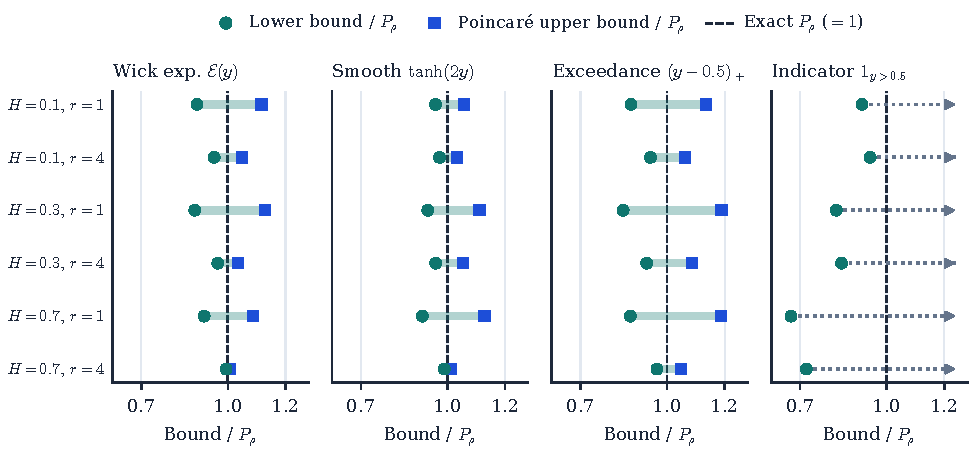
\includegraphics[width=\textwidth]{../figures/fig_v3_s1_sandwich.pdf}
\caption{Residual-to-output sandwich bounds divided by exact projection error $P_\rho$ across $24$
subordinated functional tests. Shaded bars span the lower and Poincar\'e upper bounds; the occupation
indicator has infinite gradient upper bound.}\label{fig:supp_sandwich}
\end{figure}

\subsection{Continuum coverage and monitoring bias}
Table~\ref{tab:e5c} records the complete 12-cell paired $95\%$ quantile verification for
$\int_0^1 B_H(s)^2\dd s$ across $H\in\{0.1,0.3,0.5,0.75\}$ and $n\in\{4,16,64\}$.
Figure~\ref{fig:supp_coverage} confirms that ordinary order-statistic confidence intervals targeting the
$n$-point Riemann sum fall below $90\%$ continuum coverage in \EfiveNaiveUnder\ of \EfiveCells\ cells
($0\%$ in \EfiveNaiveZero\ rough coarse cells), whereas bias-certified intervals maintain coverage
\EfiveCertMin. Figure~\ref{fig:supp_e5b} contrasts the progressive narrowing from Riemann--$W_2$ to
conditional-expectation monitoring, martingale-sharp endpoints, conditional Cantelli envelopes, and
exact binomial order statistics on identical draws.

\IfFileExists{../tables/tab_e5c.tex}{\begin{table}[!htbp]\centering\scriptsize\setlength{\tabcolsep}{3.6pt}
\caption{Paired statistical $95\%$ quantile brackets for $\int_0^1 B_H(s)^2\dd s$ from $n$-point midpoint observations ($K=20{,}000$, $100$ replications).}\label{tab:e5c}
\begin{tabular}{@{}rrrrrrr@{}}\toprule
\multicolumn{7}{@{}l}{\emph{Panel A: Grid, residual variance and empirical coverage}} \\
 & & & \multicolumn{4}{c}{Fraction of 100 replications covering the reference quantile} \\
\cmidrule(lr){4-7}
$H$ & Dates & Residual share & Martingale & Cantelli & Rao--Blackwell & Binomial Cantelli \\\midrule
0.10 & 4 & $2.4\times 10^{-1}$ & 1.00 & 1.00 & 1.00 & 1.00 \\
0.10 & 16 & $5.9\times 10^{-2}$ & 1.00 & 1.00 & 1.00 & 1.00 \\
0.10 & 64 & $1.3\times 10^{-2}$ & 1.00 & 1.00 & 1.00 & 1.00 \\
0.30 & 4 & $9.1\times 10^{-2}$ & 1.00 & 1.00 & 1.00 & 1.00 \\
0.30 & 16 & $1.2\times 10^{-2}$ & 1.00 & 1.00 & 1.00 & 1.00 \\
0.30 & 64 & $1.4\times 10^{-3}$ & 1.00 & 1.00 & 1.00 & 1.00 \\
0.50 & 4 & $2.9\times 10^{-2}$ & 1.00 & 1.00 & 1.00 & 1.00 \\
0.50 & 16 & $1.9\times 10^{-3}$ & 1.00 & 1.00 & 1.00 & 1.00 \\
0.50 & 64 & $1.2\times 10^{-4}$ & 1.00 & 1.00 & 1.00 & 0.99 \\
0.75 & 4 & $4.9\times 10^{-3}$ & 1.00 & 1.00 & 1.00 & 1.00 \\
0.75 & 16 & $1.5\times 10^{-4}$ & 1.00 & 1.00 & 1.00 & 1.00 \\
0.75 & 64 & $4.6\times 10^{-6}$ & 1.00 & 1.00 & 1.00 & 0.96 \\
\bottomrule\end{tabular}\par\medskip
\begin{tabular}{@{}rrrrrrrrr@{}}\toprule
\multicolumn{9}{@{}l}{\emph{Panel B: Median bracket widths on the same draws}} \\
 & & \multicolumn{5}{c}{DKW sampling band} & \multicolumn{2}{c}{Binomial sampling band} \\
\cmidrule(lr){3-7}\cmidrule(lr){8-9}
$H$ & Dates & Floor & Martingale & \textbf{Cantelli} & Rao--Blackwell & \shortstack{Above-floor\\ratio} & \textbf{Cantelli} & Floor \\\midrule
0.10 & 4 & 0.267 & 2.523 & \textbf{\boldmath 2.120} & 2.215 & 1.2$\times$ & \textbf{\boldmath 1.881} & 0.084 \\
0.10 & 16 & 0.299 & 1.701 & \textbf{\boldmath 1.234} & 1.321 & 1.5$\times$ & \textbf{\boldmath 1.009} & 0.094 \\
0.10 & 64 & 0.305 & 1.140 & \textbf{\boldmath 0.732} & 0.817 & 2.0$\times$ & \textbf{\boldmath 0.519} & 0.093 \\
0.30 & 4 & 0.272 & 1.791 & \textbf{\boldmath 1.353} & 1.436 & 1.4$\times$ & \textbf{\boldmath 1.138} & 0.084 \\
0.30 & 16 & 0.282 & 1.038 & \textbf{\boldmath 0.670} & 0.745 & 1.9$\times$ & \textbf{\boldmath 0.470} & 0.089 \\
0.30 & 64 & 0.282 & 0.652 & \textbf{\boldmath 0.411} & 0.489 & 2.9$\times$ & \textbf{\boldmath 0.217} & 0.089 \\
0.50 & 4 & 0.262 & 1.209 & \textbf{\boldmath 0.830} & 0.904 & 1.7$\times$ & \textbf{\boldmath 0.640} & 0.082 \\
0.50 & 16 & 0.264 & 0.644 & \textbf{\boldmath 0.410} & 0.480 & 2.6$\times$ & \textbf{\boldmath 0.229} & 0.083 \\
0.50 & 64 & 0.265 & 0.414 & \textbf{\boldmath 0.302} & 0.372 & 4.0$\times$ & \textbf{\boldmath 0.119} & 0.083 \\
0.75 & 4 & 0.242 & 0.709 & \textbf{\boldmath 0.461} & 0.522 & 2.1$\times$ & \textbf{\boldmath 0.292} & 0.076 \\
0.75 & 16 & 0.239 & 0.384 & \textbf{\boldmath 0.277} & 0.340 & 3.9$\times$ & \textbf{\boldmath 0.112} & 0.074 \\
0.75 & 64 & 0.238 & 0.283 & \textbf{\boldmath 0.245} & 0.308 & 6.6$\times$ & \textbf{\boldmath 0.082} & 0.076 \\
\bottomrule\end{tabular}
\smallskip\par\raggedright\scriptsize\emph{Notes:} Bold identifies \RoughCertCV{} Cantelli widths with Dvoretzky--Kiefer--Wolfowitz (DKW) bands or exact binomial order statistics. Rao--Blackwell integrates out auxiliary randomness. The floor measures sampling uncertainty of the conditional monitor alone. The above-floor ratio divides martingale excess width by Cantelli excess width. Residual share is unexplained variance divided by total variance.
\end{table}
}{}

\begin{figure}[!htbp]\centering
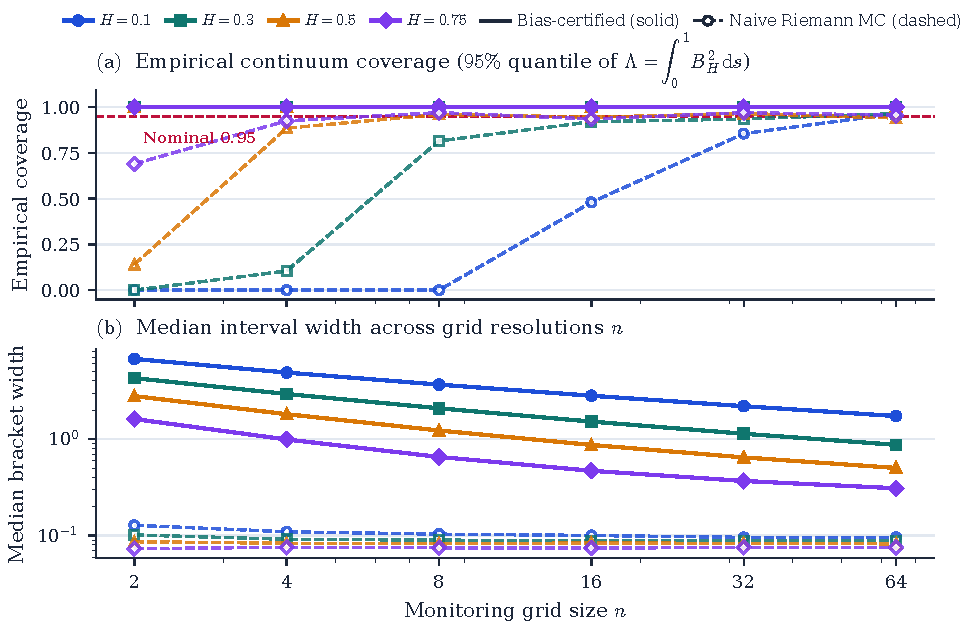
\includegraphics[width=\textwidth]{../figures/fig_v3_s2_coverage.pdf}
\caption{Empirical coverage (a) and median width (b) of $95\%$ continuum quantile intervals for
$\int_0^1 B_H(s)^2\dd s$ versus grid size $n$ ($K=20{,}000$). Dashed line marks nominal $0.95$ coverage.}
\label{fig:supp_coverage}
\end{figure}

\begin{figure}[!htbp]\centering
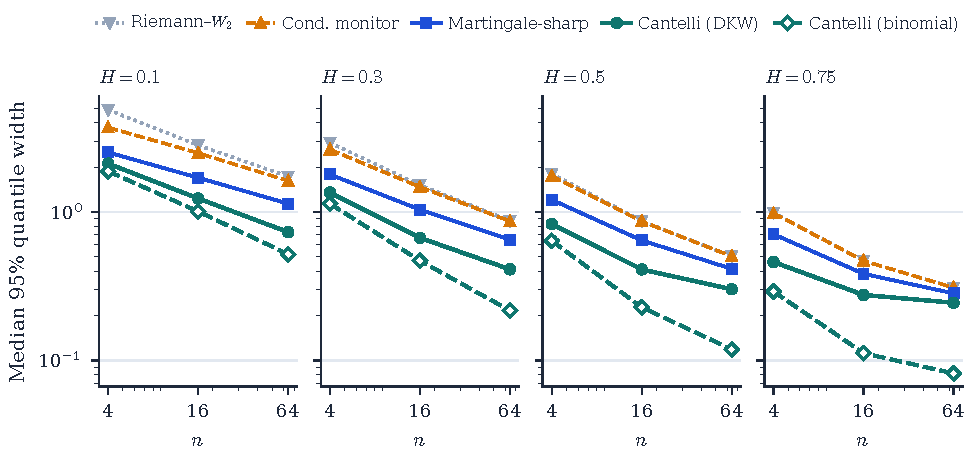
\includegraphics[width=\textwidth]{../figures/fig_v3_s3_layers.pdf}
\caption{Progressive width reduction across certificate layers for the $95\%$ quantile of
$\int_0^1 B_H(s)^2\dd s$ on identical samples: Riemann--$W_2$, conditional monitor, martingale-sharp,
and conditional Cantelli brackets with DKW (solid) and exact binomial order statistics (dashed).}\label{fig:supp_e5b}
\end{figure}

\subsection{Measured monitoring convergence rates}
We evaluated the monitoring error $M(\mu_n)$ using Theorem~1 of the main paper and fitted slopes on
midpoint grids $n=64,128,256,512,1024$. For Wick exponentials the comparison rate is
$n^{-(1+2H)}$ in the range of Theorem~3: the fitted slopes are $-\SlopeWickA$, $-\SlopeWickB$,
$-\SlopeWickC$ and $-\SlopeWickD$ at $H=0.1,0.3,0.5,0.7$, against the predicted $-1.2$, $-1.6$, $-2.0$
and $-2.4$. The kinked exceedance and discontinuous indicator are additional numerical tests, with
empirical slopes compared against $-(1+2H)$ and $-(1+H)$, respectively
\citep{Altmeyer2017,NgoOgawa2011}: the exceedance gives $-\SlopeKinkA$, $-\SlopeKinkB$, $-\SlopeKinkC$
and $-\SlopeKinkD$, the indicator $-\SlopeIndA$, $-\SlopeIndB$, $-\SlopeIndC$ and $-\SlopeIndD$, and the
generic $\tanh(2y)$ functional $-\SlopeTanhA$, $-\SlopeTanhB$, $-\SlopeTanhC$ and $-\SlopeTanhD$ over the
same grids.
\FloatBarrier

\section{Additional pricing and verification details}
For the mixed smile we bisect $Y(z)-K^2$ on $[-16,16]$ and integrate on the exercised
side using complex ball quadrature. The unresolved root interval is covered by its length
times a supremum bound. All three Hermite-weighted terms use the same exercise root.
For $s_{\max}<8$ and $|z|\ge16$, the absolute integrand, including the normal density,
is bounded by $A(1+z^2)e^{-z^2/4}/\sqrt{2\pi}$, where
\[
 A=K+\sqrt{\bar\xi}\left(1+\sum_j
 (|\gamma_{1,j}|+|\gamma_{2,j}/s_j|+2|\gamma_{3,j}/s_j^2|)\right).
\]
We integrate this majorant over both tails. The tail follows from $\mu_j\le0$,
$0\le y_j/\sqrt{Y}\le\sqrt{Y}$ and
$\sqrt{Y}\le\sqrt{\bar\xi}\exp(s_{\max}|z|/2)$. For the independent finite-difference
calculation the original $100$-node Gauss--Hermite rule and $10^{-4}$ step are passed to the authors'
function. On the same fixed strikes we invert each price with its own forward.

\paragraph{Functional quantisation}
On $L=T+\Delta$, put $\omega_j=(j-1/2)\pi/L$. The retained loading is
$\sqrt{2/L}\int_0^T (T+x-s)^{-p}\cos(\omega_j s)\dd s$, with $p=1/2-H$.
Writing $b=1-p$, the antiderivative of $t^{-p}e^{-i\omega_jt}$ starting at zero is
$t^b\,{}_1F_1(b;b+1;-i\omega_jt)/b$. Taking the real part after translation yields
the loadings used for product quantisation in \citet{BonesiniCallegaroJacquier2023}.
Scalar Gaussian codepoints satisfy the centroid equations with Voronoi thresholds given
by adjacent midpoints. Each conditional mean increases with either endpoint.
Verifying lower and upper sub- and supersolutions maps the entire ordered box into itself.
Existence follows by the fixed-point theorem on a compact box, and strict log-concavity
gives uniqueness of the stationary scalar normal quantiser. We recompute the Voronoi
masses in ball arithmetic. The price integral for every path uses its full deterministic
variance compensation. Absolute derivatives of a mode on $x>0$ are bounded by
$\sqrt{2/L}\,x^{-p}$ and $\sqrt{2/L}\,p x^{-p-1}$, respectively, by integrating
the kernel derivatives. On the first cell the loading variation is bounded by
$\sqrt{2/L}\,(x_1^{1-p}-x_0^{1-p})/(1-p)$.
Every online price sum includes the uncertainty of both centroids and masses.

\paragraph{Finite-dimensional kernels and the tilted contrast}
Writing $r(x)=(w_i e^{-\gamma_i x})_i$, the Gram matrix of the exponential factors has entries
$G_{ij}=\int_0^T e^{-(\gamma_i+\gamma_j)t}\dd t$.
The covariance is $r(x)^\top G r(y)$. Componentwise positivity gives the required
derivative suprema at left endpoints. For the more demanding threshold at $H=0.05$,
we tilt by $h=0.99\,\Delta^{-1}\int k_x\dd x$ and condition under the new measure on
the unit vector $e$ proportional to $k_{\Delta/14}-k_\Delta$. The residual loading becomes
$g(x)=\langle k_x-h,e\rangle$ and its variance comes from the Gram matrix of
$(I-e\otimes e)(k_x-h)$. Since $e$ is positive in Brownian time, $g$ decreases.
The weight now includes $\exp(-\langle h,k_x-h\rangle/2)$. For its Gaussian-weighted
integrand the log derivative is bounded by
$(|z-g|+\|h\|/2)\|k_x'\|$; the log second derivative is bounded by
$(|z-g|+\|h\|/2)\|k_x''\|+\|k_x'\|^2$. The same cell and panel remainders then apply.
The tilted tail uses the bound $\sqrt{m_1\Pr(|Z|>10)}$ before multiplication by
$e^{-\|h\|^2/8}$. This calculation encloses each price separately.

\paragraph{Simulation check}
A second program builds the Brownian loadings directly using 224 graded quadrature nodes,
then factorises the resulting delivery covariance by SVD. It pairs the payoff with the
conditional lognormal sum on the leading coordinate. The expectation of that control is
computed by root-split one-dimensional quadrature. We use 48 and 96 delivery nodes and
$2^{14}$ and $2^{17}$ Sobol paths per scramble, respectively. Twelve independent scrambles
give replicate standard errors. Discretisation and discarded singular values remain
numerical approximations. Agreement with the deterministic bands is a diagnostic. A second implementation forms the delivery covariance from a hypergeometric primitive at 130 decimal digits, computes a Cholesky factor at 40 delivery nodes, then samples all 40 Gaussian coordinates with independent scrambles. Its 35 point estimates also fall inside their respective bands.

{\small
\setlength{\bibsep}{3pt}
\bibliographystyle{elsarticle-num-names}
\bibliography{../references}
}
\end{document}

